\section{Drop out}
\paragraph{Purpose}
It provides an inexpensive approximation to \tB{training and evaluating a \emph{bagged
ensemble} of exponentially many neural networks}.

\paragraph{Theory}
It \uB{trains the ensemble consisting of \textbf{all sub-networks that can be formed by
removing non-output units}} from an underlying base network.\\
At each training step, every unit of a layer is kept independently with probability
$p$ (\emph{keep probability}): with a mask $\bm{\mu}$ whose entries are i.i.d.
$\mathcal{B}(p)$, the layer output becomes $\tilde{\bm{h}} = \bm{\mu}\odot\bm{h}$.
Typical values are $p=0.5$ for hidden units and $p=0.8$ for input units.

\paragraph{Inference} At test time all units are kept, so the expected input of the next
layer would be $\frac{1}{p}$ times larger than during training. Two equivalent fixes:
\begin{itemize}
    \item \textbf{weight scaling inference rule}: multiply the weights by $p$ at test time;
    \item \textbf{inverted dropout} (the common implementation): divide the kept
        activations by $p$ during training, and leave the network unchanged at test time.
\end{itemize}

\paragraph{Differences with bagging} In bagging the models are independent and trained
to convergence. With dropout the sub-networks \tB{share parameters} and each one is
trained for a single step, if it is even sampled.\\
Dropout is also used in Transformers, where it is applied to the output of each
sub-layer before the residual connection (original paper: $P_{drop}=0.1$).
\begin{figure}[H]
    \begin{center}
        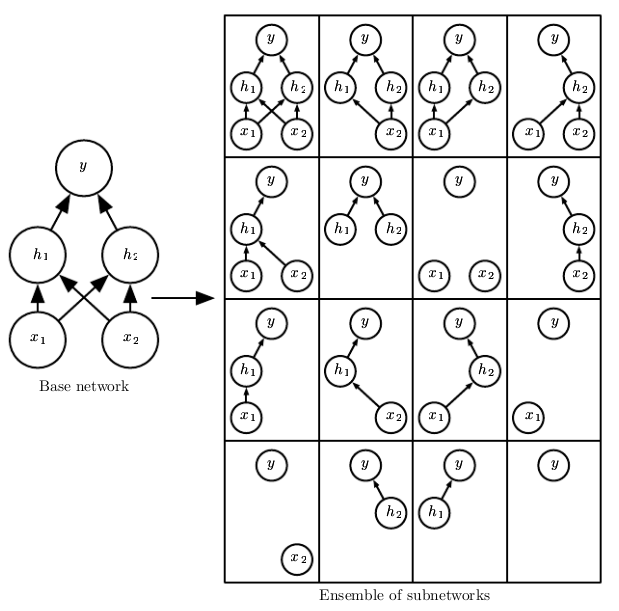
\includegraphics[width=.5\textwidth]{chapters/4_deep_learning/2_regularization/images/01_droupout.png}
    \end{center}
    \caption{Drop out illustration}
    \label{fig:01_droupout.png}
\end{figure}
